
\chapter{Background}\label{C:background}

This projects work is an extension of the existing state of the art, the Restricted Boltzmann Machine and therefore the origins and work related to Restricted Boltzmann Machines (RBMs) will occur in section \ref{S:RBM}. First, an example to ground this discussion will be given; the Cocktail Party Problem.

\section{The Cocktail Party Problem}\label{SS:CPP}

The Cocktail Party Problem as explored by McDermott J. in \cite{McDermott:2009cs}, nicely illustrates the concept of Blind Source Separation. Blind Source Separation is, as the name implies, is being able to take a noisy multi-cause input and separate it out into the underlying causes or 'sources'.

The Cocktail Party Problem centres on the way a partygoer can focus on a single conversation, despite there being multiple conversations going on in the background. The listener has to distinguish, given the mixed audio signal, the underlying conversation of interest. 

The Cocktail Party Problem is applicable to the goals of the approach this project explores. The approach aims to leverage an understanding of the different models, or in the context of this problem, separating the sources. 

\section{The Restricted Boltzmann Machine}\label{S:RBM}

As touched on in the context section \ref{S:introcontext}, extending Restricted Boltzmann Machine forms the basis of the project. In this section the RBM will be explained with enough detail to understand at a high level how the theory being tested works. It is not in scope of this project to provide the proof for the theory.

The RBM  was originally  conceived by Smolensky P under the name 'Harmonium' \cite{Smolensky:1986vy}  in 1986. The example Smolensky presents as a 'cognitive task' that the RBM could solve is similar to that in which this project is focused; identifying an image of text with parts obscured, effectively separating the sources by ignoring the obscuring noise.

Hinton G. brought the Restricted Boltzmann Machine back into popularity recently, via a new tractable training technique \cite{Hinton:2006dk}. This allows training in a greedy fashion where the individual units of the representation are independent. This means a hidden representation can be generated in a single pass. This is important because given a rich dataset like an audio signal in the Cocktail Party Problem, a single pass limits the complexity of training to be the number of times you run over the dataset.

\begin{figure}[htbp]
\begin{center}
	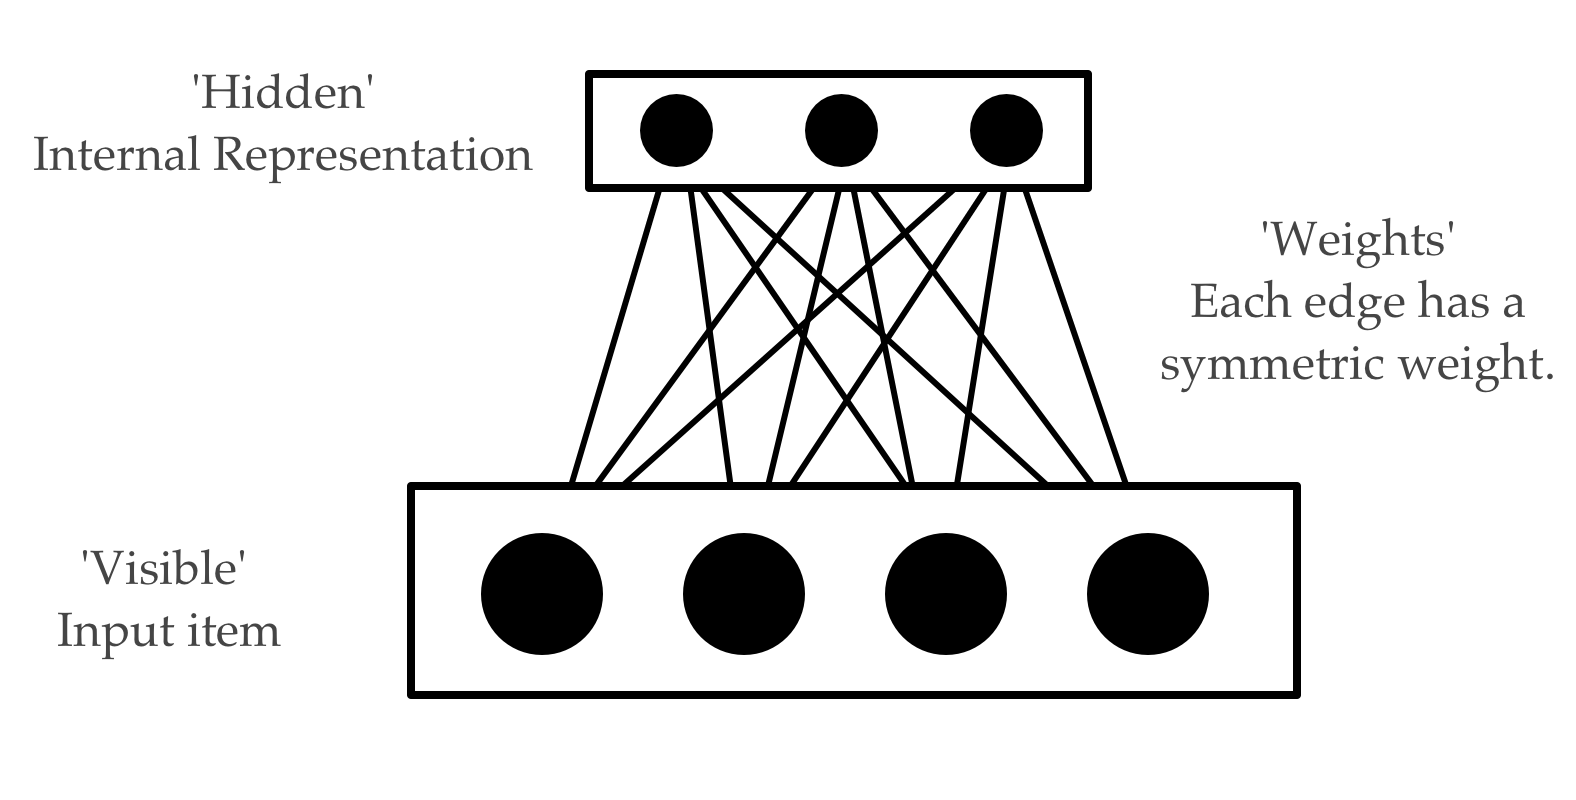
\includegraphics[width=0.7\textwidth]{Assets/RBMimage}
\caption{Visual representation of an RBM.}
\label{F:rbm}
\end{center}
\end{figure}

The new approach sacrifices this single pass with the aim to construct a more representative internal model of multi-cause input data compared to the traditional approach. This requires an understanding of the RBMs structure which is akin too that of a fully connected bipartite graph. In the RBM, the edges between the groups of nodes each have an associated 'weight'. These weights are tweaked during the training process to maximise the probability of generating the best representation of all the data items in the training set. 

Fig \ref{F:rbm} shows a graphical representation of an RBM, in this case with three hidden units and four visible units. Each edge between the visible and hidden layers has a symmetric weight. This weight is used to transform one layer's (visible or hidden) representation to the other. Both the visible and hidden units are binary, i.e. $ \in {0,1} $.

\subsection{Internal Representation}\label{SS:repr}

The new approach takes the form of having two Restricted Boltzmann Machines, one trained on the entity of interest, another on noise. 
This amounts to slightly changing the way the internal representation is generated for a given input vector. In the context of images, say a single digit CAPTCHA, this approach aims to allow the digit model to take responsibility for the parts of the images that look like a digit. Conversely, the noise model is able to take responsibility for parts of the image that look like noise. 

The internal representation of the input for RBMs is described below.
Given an RBM with $j$ hidden units (for representing the input), $i$ input units, and weights matrix $W_{ji}$ that represent the symmetric weights between the input and the representation, we want to find the internal representation for all $ h_j $ units given an input vector $ \tilde{v} $.
First the weighted sum into a given hidden unit is calculated via 
$$ \psi_j = \sum_i ( W_{ji}v_i ) $$
A Bernoulli trial is performed to see if based on $ \psi_j $, the hidden unit $ h_j $ gets set to 1 or 0.
Let $ x  $ be a random floating point such that $ x \in [0-1] $.
$$ P(h_j = 1 | \tilde{v}) = 
\begin{cases} 
  \sigma(\psi_j) > x & 1 \\
  \sigma(\psi_j) \leq x & 0
\end{cases} $$
Here we see the logistic or sigmoid function $\sigma$. This acts as a smooth threshold for deciding whether to turn on the hidden unit.

\subsection{New Approach}

The new approach introduces a second RBM. so a change in notation is required. A subscript or superscript $A$ or $B$ can be added to all the values defined above to specify they come from $model_A$ or $model_B$ respectively. The update to the hidden units of $model_A$ is as defined above, with a slight change to the calculation of $\psi_j$:

$$ \psi_j = \sum_i ( W_{ji}v_i ) + \sum_i (C^A_{ji}) $$

Where $ C^A_{ji} $ is the correction that is applied, this is where the interaction between the two RBM's takes place allowing one to take responsibility for different parts of the input.
The proof of this theorem is not in the scope of the project, however the definition for $ C^A_{ji} $ can be briefly discussed. It is defined as:

$$C^A_{ji} \; = \;\log \bigg[ \frac{\sigma (\phi_i^{j=0})}{\sigma (\phi_i^{j=1})} . \frac{\sigma (\phi_i^{j=1} + \epsilon_i) }{\sigma (\phi_i^{j=0} + \epsilon_i)} \bigg] $$

Where $ \phi_i $ is the weighted sum into the $ith$ visible node. $\phi_i^{j=0} $ is the weighted sum into the $ith$ visible node without any contribution from the weight $ W_ji $. Conversely, $ \phi_i^{j=1} $ is the weighted sum into the visible node $i$ where the $jth$ hidden node is turned on; its weight contributing to the weighted sum. Finally, $ \epsilon $ is the contribution from the 'other' RBM. It is the weighted sum into the $ith$ visible unit from the other RBM. 

This correction adds an expensive calculation to generating the hidden representation. Unfortunately, it introduces dependancy between the hidden units, meaning we have to repeat this calculation $x$ number of times so the probabilities of turning off/on the hidden units can reach equilibrium.






